\section{Circumcircle family}

This family is inscribed in a circle of radius $R$ centered on $O=X_3$ and circumscribes a concentric ellipse with semi-axes $a,b$; see     \cref{fig:06-six-caps}(top right). Recall that the Cayley condition implies $R=a+b$. 

\begin{proposition}
Over circumcircle 3-periodics, the locus of the barycenter $X_2$ is a concentric circle with radius $r_2$ given by:

\[ r_2 = \frac{1}{3}(a-b)  \]

\end{proposition}

Referring to \cref{fig:06-circum-x1456-loci}:

\begin{proposition}
Over circumcircle 3-periodics, the loci of both the orthocenter $X_4$ and the center $X_5$ of the 9-point circle are concentric circles centered on $X_3$, with radii $2 d'$ and $d'$ respectively, where $d'=(a-b)/2$ .
\label{prop:06-circum-x1456-loci}
\end{proposition}

\begin{proof}
Based on 3-periodic vertex parametrization and CAS-assisted algebraic simplification.
\end{proof}

\begin{figure}
    \centering
    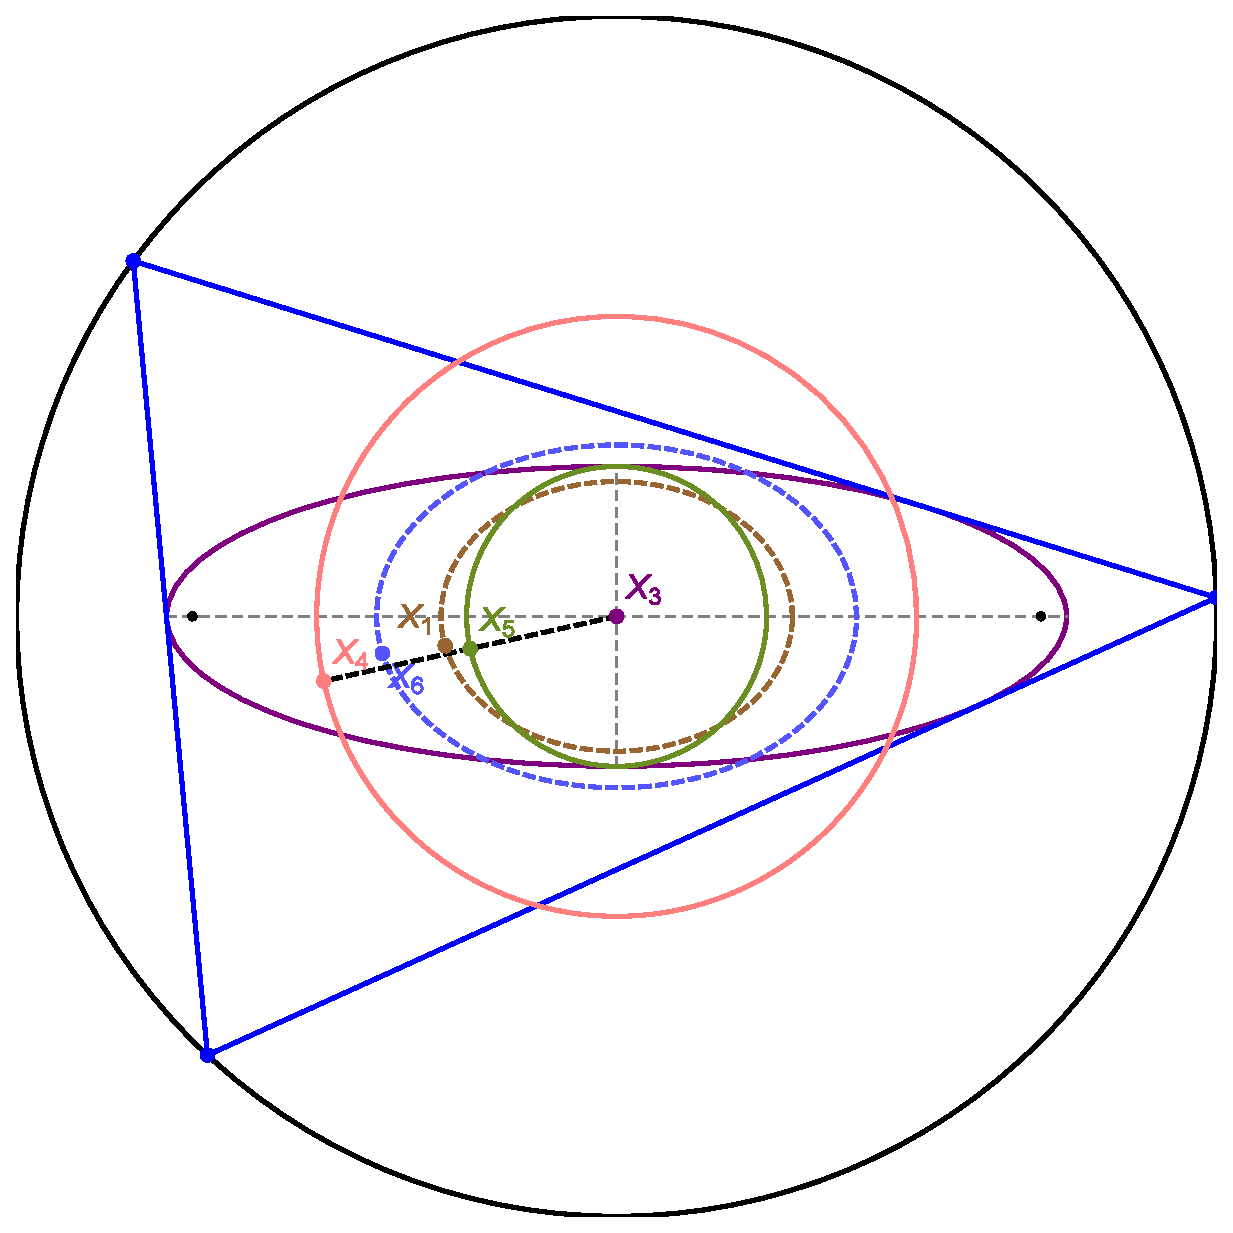
\includegraphics[width=.7\textwidth]{pics_06_030_system_II_locus.eps}
    \caption{A circumcircle 3-periodic: The loci of both orthocenter $X_4$ (pink) and nine-point center $X_5$ (olive green) are concentric with the external circle (black). Their radii are $2d'$ and $d'$, respectively where $d'=|X_4-X_5|$. In contradistinction to the elliptic billiard, the locus of the incenter $X_1$ (dashed brown) is non-elliptic while that of the symmedian point $X_6$ (dashed blue) is an ellipse. \href{https://youtu.be/8xlYaQfQCTw}{Video}, \href{https://bit.ly/3vo8eWl}{Live}}
    \label{fig:06-circum-x1456-loci}
\end{figure}

Recall that in the confocal pair the locus of $X_1$ (resp. $X_6$) is an ellipse (resp. a quartic) \cite{garcia2020-ellipses}; see Appendix~\ref{app:loci-x1x6}. Interestingly:

\begin{proposition}
Over circumcircle 3-periodics, the locus of the symmedian point $X_6$ (resp. the incenter $X_1$) is an ellipse (resp. the convex component of a quartic -- note the other component corresponds to the locus of the 3 excenters which can be concave). These are given by:

\begin{align*}
\text{locus of $X_6$}: &\; \frac{x^2}{a_6^2}+\frac{y^2}{b_6^2}=1, \; a_6=\frac{ a^2 - b^2}{a + 2 b},\;\;  b_6=\frac{ a^2 - b^2}{2a +  b},\\
\text{locus of $X_1$}:&\; \left( {x}^{2}+{y}^{2} \right) ^{2}-2\, \left( a+3\,b \right) 
 \left( a+b \right) {x}^{2}-2\, \left( a+b \right)  \left( 3\,a+b
 \right) {y}^{2} \\
 &+\left( a^2-b^2 \right) ^{2}=0\cdot
 \label{thm:II-loci_X1}
\end{align*}
\end{proposition}

\begin{proof}
CAS-assisted simplification.
\end{proof}

